\section{Genauigkeit}
Die Genauigkeit des Programms ist stark abhängig von der Genauigkeit unsere log2-Implementierung. Für die log2-Approximationen können wir für die Genauigkeit eine analytische Untersuchung durchführen. Wir sind auf die Differenz zwischen log2 und unseren Approximationen der log2 interessiert. Dann finden wir die Ableitung der Differenz, um das Maximum/Minimum im Bereich von 1 bis 2 herauszuziehen.  

\subsubsection*{Log2 Approx DEG2 -- $P_{2}(x)$ \eqref{eq:deg2}}

\begin{equation*}
    (\mathrm{log_{2}}(x) - \mathrm{P_{2}}(x))'
    = \frac{1}{x \cdot \ln(2)} + 0.68969 \cdot x - 2.024658
\end{equation*} \par

Nullstellen: $x_{1} \approx 1.718089, x_{2} \approx 1.217517$ \par

Der größte absolute Fehler für diese Approximation ist ungefähr $4.941 \cdot 10^{-3}$.

\subsubsection*{Log2 Approx DEG4 -- $P_{4}(x)$ \eqref{eq:deg4}}

\begin{equation*}
    (\mathrm{log_{2}}(x) - \mathrm{P_{4}}(x))'
    = \frac{1}{x \cdot \ln(2)} + 0.32646 \cdot x^{3}
    - 1.93543 \cdot x^{2} +4.24135 \cdot x - 4.07009
\end{equation*} \par

Nullstellen: $x_{1} \approx 1.08506,  x_{2} \approx 1.31912, x_{3} \approx 1.62916, x_{4} \approx 1.89513$ \par

Der größte absolute Fehler für diese Approximation ist ungefähr. $8.752644 \cdot 10^{-5}$.

\subsubsection*{Log2 Approx ARTANH -- $S_{2}(x)$ \eqref{eq:artanh}}

\begin{equation*}
    (\mathrm{log_{2}}(x) - \mathrm{S_{2}}(x) \cdot \frac{1}{ln(2)})'
    = \dfrac{x^6-6x^5+15x^4-20x^3+15x^2-6x+1}{\ln\left(2\right)x\left(x+1\right)^6}
\end{equation*} \par

Nullstellen: $x = 1$ \par

Auf die Stelle x gleich 1 ist die Differenz 0. Aber, der größte Wert im Bereich findet sich auf die Stelle x = 2, weil der Funktion steigend ist. Der größte absolute Fehler für diese Approximation ist ungefähr $2,063996 \cdot 10^{-4}$.

\begin{figure}[h]
    \label{fig:absolute-mistake}
  \centering
  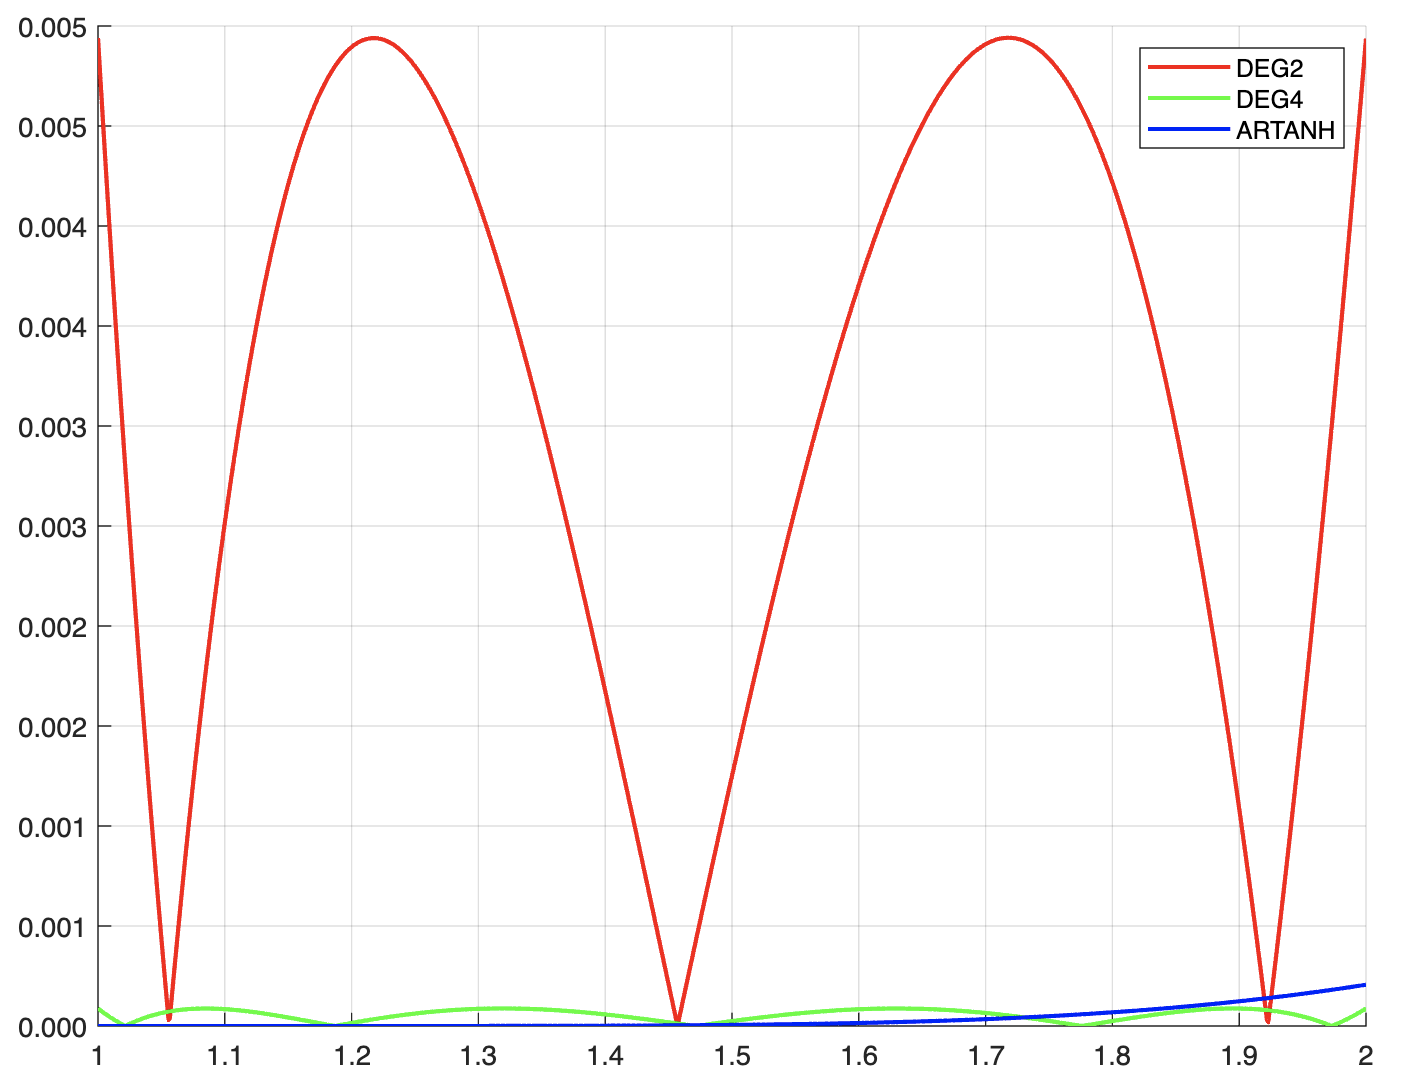
\includegraphics[scale=0.35]{abs_mistake.png}
  \caption{Absolute Fehler der Logarithmusfunktionen im $[1,2)$}
\end{figure}

Wir erwarten, dass die DEG4-Approximation uns bessere Ergebnisse liefert, weil es den kleinsten Fehler hat. (Siehe Abbildung \ref{fig:absolute-mistake})

Wir haben nur den maximalen absoluten Fehler für die log2 im Bereich [1,2] berechnet. Am Ende wird der Fehler für die log2 Approximation noch kleiner, weil diese Zahl mit dem log2 vom Exponenten addiert wird. Der log2 des Exponenten ist im Intervall [-126,0] und der log2 der Mantisse ist im Intervall [0,1]. Daher sinkt der relative Fehler mit der Addition. Der Fehler für die Lookup Version der log2 mit der empfohlene 16-Bit-Mantisse ist $6.55 \cdot 10^{-6}$.~\cite{fast_log}
% Der absolute Fehler sinkt auch (in Vergleich zu andere 32 Bit Fließkommaberechnung), weil bei der Addition Auslöschung auftritt, und das kann potenziell falsch berechnete Stellen der log2 der Mantisse entfernen. \\


Die Berechnung der Entropiefunktion enthält eine Multiplikation von der Logarithmusfunktion mit einem Wert $x$, der immer kleiner gleich 1 ist, welches die Abnahme des absoluten Fehlers verursacht.

Bei einer naiven Implementierung der Entropiefunktion gibt es auch einen Unterschied in Genauigkeit zwischen der Skalar- und SIMD-Version der Entropie. Wobei der SIMD Version genauer ist. Da der SIMD Version 4 Teil-summen berechnet, werden weniger Additionen von Auslöschung beeinflusst. Immer noch haben wir bemerkt, dass in beiden Fällen unsere Ergebnisse sehr stark von Auslöschung beeinflusst wurden.

\begin{figure}[h]
\centering
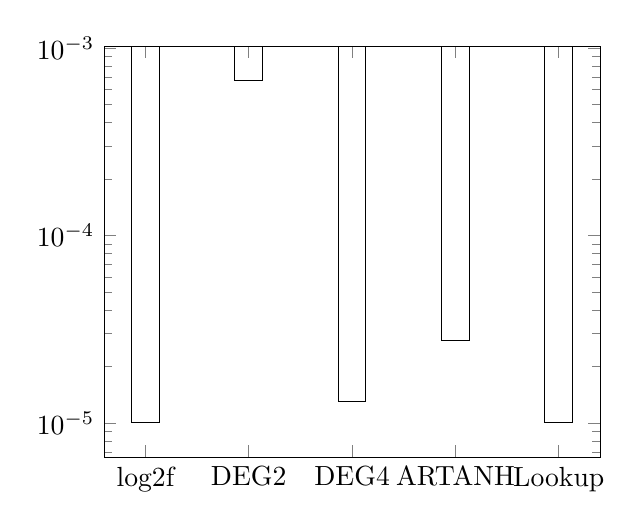
\begin{tikzpicture}
    \begin{axis}[
        symbolic x coords={log2f, DEG2, DEG4, ARTANH, Lookup},
        xtick=data,
        ymode = log,
        width = \textwidth *0.65
      ]
        \addplot[ybar] coordinates {
            (log2f,   0.000010)
            (DEG2,  0.000671)
            (DEG4,   0.000013)
            (ARTANH, 0.0000275) 
            (Lookup, 0.000010)
        };
    \end{axis}
\end{tikzpicture}
\caption{Entropiefehler Größenordnung (Durchschnitt bei zufälligen Daten)}
\end{figure}

Wie schon erwähnt in dem Ansatz, nutzen wir die Kahan-Summe~\cite{kahan}, um Auslöschung zu vermeiden. Die Kahan-Summe speichert der unbehandelte Teil  einer Addition in die Variable Kompensation und bei der nächste Addition wird die Kompensation aufaddiert. Die Kahan-Summe nimmt an, dass die Summe größer als der nächste zu addierende Zahl ist. Diese Annahme gilt bei uns auch. Wenn wir die Kahan-Summe verwenden sind die Ergebnisse bei SIMD und Skalar fast gleich.